% Para compilar, use:
% pdflatex -shell-escape lindasapresentacoes.tex
%%%%%%%%%%%%%%%%%%%%%%%%%%%%%%%%%%%%%%%%%%%%%%%%%%%%%%%%%%%%%%%%%%%%%%%%%%%%%%%%%%%%%%%%%
% PREAMBULO
%%%%%%%%%%%%%%%%%%%%%%%%%%%%%%%%%%%%%%%%%%%%%%%%%%%%%%%%%%%%%%%%%%%%%%%%%%%%%%%%%%%%%%%%%
\documentclass{beamer}
% Temas do beamer
\usetheme{default}
\useinnertheme[shadow=true]{rounded}
\usefonttheme[onlysmall]{structurebold}
% This Charming Man palette from colorlovers.com
\definecolor{grrey}{rgb}{0.2,0.2,0.2}
\definecolor{allcs}{rgb}{0.8,0.8,0.8}
\definecolor{handsomedevil}{rgb}{0.549,0.192,0.188}
\definecolor{submerged}{rgb}{0.262,0.47,0.619}
% Escolhendo as cores padrão do beamer
\setbeamercolor{normal text}{fg=grrey}
\setbeamercolor{structure}{fg=grrey}
\setbeamercolor{block title}{fg=handsomedevil,bg=allcs}
\setbeamercolor{block body}{bg=allcs}
\setbeamercolor{alerted text}{fg=handsomedevil}
\setbeamercolor{frametitle}{fg=handsomedevil!90!allcs}
% Customizações
\setbeamertemplate{title page}
{%
   \vspace{5.3cm}\color{white}
   \begin{flushright}
      \Huge{\bfseries\inserttitle}\\
      \large{\insertauthor}\\
      \small{\insertdate}
   \end{flushright}
}
\setbeamertemplate{footline}
{%
   \begin{beamercolorbox}[wd=.333333\paperwidth,ht=2.25ex,dp=1ex,right]{}
   \end{beamercolorbox}
}
\pgfdeclarehorizontalshading[frametitle.bg,frametitle right.bg]{beamer@frametitleshade}{\paperheight}{%
  color(0pt)=(frametitle.bg);
  color(\paperwidth)=(frametitle right.bg)}
\AtBeginDocument%
{
  \pgfdeclareverticalshading{beamer@topshade}{\paperwidth}{%
    color(0pt)=(bg);
    color(4pt)=(black!50!bg)}
  \pgfdeclareverticalshading{beamer@bottomshade}{\paperwidth}{%
     color(0pt)=(black!50!bg);
     color(4pt)=(bg)}
}
\addtobeamertemplate{headline}
{}
{%
  \vskip-0.2pt
  \pgfuseshading{beamer@topshade}
  \vskip-2pt
}
\addtobeamertemplate{footline}
{}
{%
  \vskip-2pt
  \pgfuseshading{beamer@bottomshade}
}
\setbeamerfont{frametitle}{family=\bfseries}
\AtBeginSection{\frame{\tableofcontents[currentsection,hideallsubsections]}}
%
% Pacotes adicionais
\usepackage[utf8]{inputenc} % Para permitir a exibição correta de acentos
\usepackage[portuguese]{babel} % Para exibir palavras-chave em português
\usepackage{txfonts} % Fontes bonitas :)
%
\usepackage{listings} % Para mostrar código com realce de sintaxe
\lstset{ %
   basicstyle=\footnotesize\ttfamily\color{grrey},
   escapeinside={\%*}{*)},          % para exibir comandos LaTeX
   keywordstyle=\bfseries\color{submerged}, % cor das palavras-chave
   language={[LaTeX]tex},
   % Para formatar mais palavras como keywords
   morekeywords={*,framezoom,includegraphics,alert,uncover,only,alt,%
      temporal,usetheme,usecolortheme,useinnertheme,usefonttheme,useoutertheme},
   showstringspaces=false,          % não mostrar underline no lugar de espaços
   tabsize=2,                       % sets default tabsize to 2 spaces
   escapechar={€},% needed to set tikz anchors in listings
   xleftmargin=\parindent,
   belowskip=1pt,
   boxpos=c,
   extendedchars=\false,
}
%
% TiKZ
\usepackage{tikz}
\usetikzlibrary{shapes,arrows} % Biblioteca de formas do TikZ

% Novo macro para exibir palavras chave em cores
\newcommand{\kw}[1]{\textbackslash {\color{submerged}#1}}

% Variáveis da apresentação
\title{Lindas apresentações\\ com o \LaTeX}
\author{Melissa Weber Mendonça}
\date{SoLiSC 2013}

%%%%%%%%%%%%%%%%%%%%%%%%%%%%%%%%%%%%%%%%%%%%%%%%%%%%%%%%%%%%%%%%%%%%%%%%%%%%%%%%%%%%%%%%%
% FIM DO PREAMBULO
%%%%%%%%%%%%%%%%%%%%%%%%%%%%%%%%%%%%%%%%%%%%%%%%%%%%%%%%%%%%%%%%%%%%%%%%%%%%%%%%%%%%%%%%%

\begin{document}

{% Definindo frame de título.
   \setbeamertemplate{footline}{} 
   \setbeamertemplate{headline}{}
   \usebackgroundtemplate{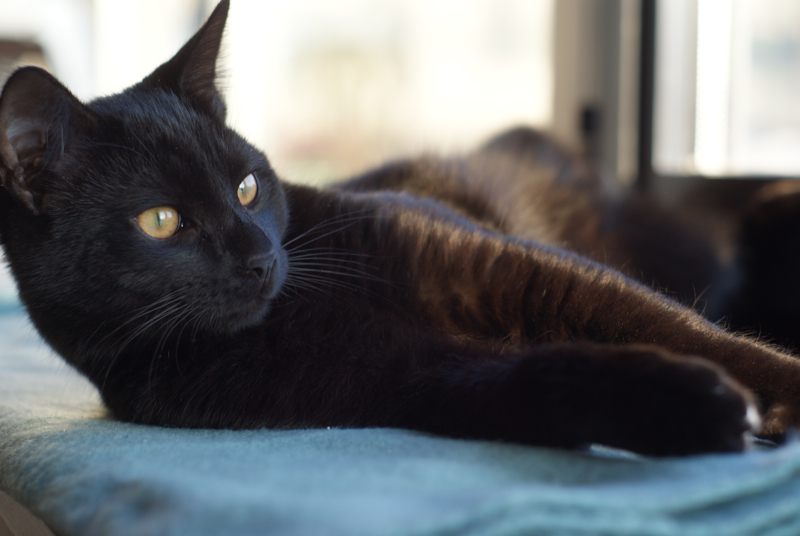
\includegraphics[width=\paperwidth,height=\paperheight]{imagens/linus.jpg}}%
\begin{frame}%
   \titlepage%
\end{frame}%
}

\begin{frame}
   \frametitle{Por que fazer apresentações bonitas?}
   \begin{center}
      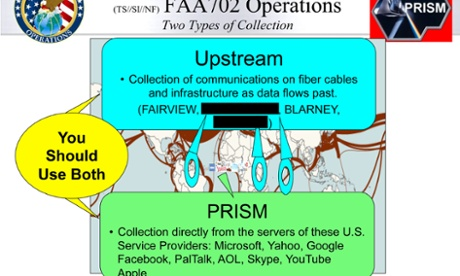
\includegraphics[width=7cm]{imagens/prism.jpeg}
   \end{center}
   Ser descuidado com suas apresentações pode comunicar falta de interesse, descaso e até \alert{desrespeito} com sua audiência.
\end{frame}

\begin{frame}
   \frametitle{Roteiro}
   \tableofcontents[pausesections]
\end{frame}

\section{Básico}

\subsection{\LaTeX, Beamer}

\begin{frame}
   \frametitle{O que é \LaTeX ?}
   \begin{columns}
      \column{6cm}
      \begin{overlayarea}{6cm}{7cm}
         O \LaTeX\ é um sistema de composição tipográfica de alta qualidade.

         \begin{center}
            \begin{block}{}
               \begin{center}
                  Conteúdo $\ne$ Forma
               \end{center}
            \end{block}
         \end{center}         
         \vspace{1cm}
         \begin{center}
            \only<2>{\alert{\LaTeX\ é software livre!}}
         \end{center}
      \end{overlayarea}
      \column{3.5cm}
      \begin{center}
         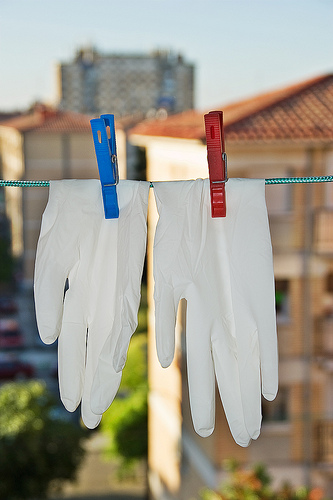
\includegraphics[width=3.5cm]{imagens/latex.jpg}
         % Photo Credit: http://www.flickr.com/photos/11080284@N02/5940374090/ (Anvica) via Compfight CC-by-nc-nd/2.0 
      \end{center}
   \end{columns}
\end{frame}

\begin{frame}
   \frametitle{Beamer}
   \setbeamercovered{transparent}
   \begin{block}{}
      Classe de documento \LaTeX\ usada para criar apresentações.
   \end{block}
   \vspace{0.5cm}
   Vantagens:
   \begin{itemize}
      \item<2-> Gera arquivos PDF de tamanho modesto.
      \item<3-> Temas básicos bonitos e funcionais
      \item<4-> Numeração automática de seções, capítulos, figuras, tabelas, equações, etc
      \item<5-> Citação automática de itens bibliográficos
      \item<6-> Programável/Customizável
      \item<7> \emph{Output} variável: tela, \emph{handouts}, notas.
   \end{itemize}
\end{frame}

\begin{frame}
   \frametitle{Procedimento padrão}
   \begin{columns}
      \column{6cm}
      \begin{itemize}
         \item Escrever código no editor e salvar num arquivo com extensão {\tt{.tex}}
         \uncover<2->{\item Compilar: \\{\tt{pdflatex arquivo.tex}}}
         \uncover<3->{\item Visualizar PDF}
      \end{itemize}
      \column{4cm}
      \begin{tikzpicture}[node distance=2cm, overlay]
         \node (editor) at (1.5,1.5) {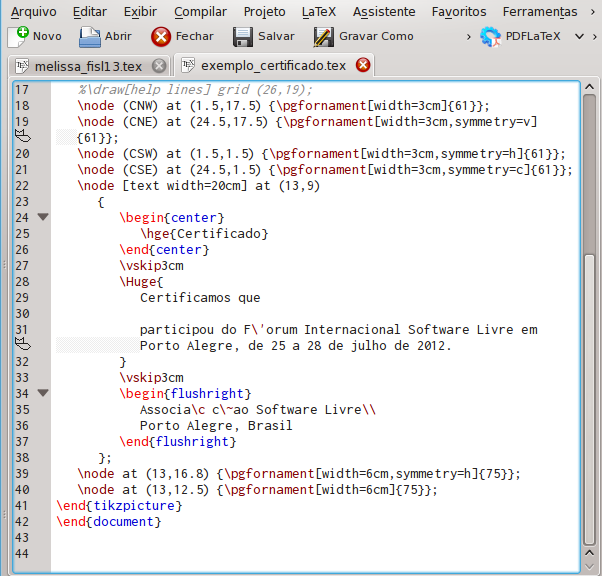
\includegraphics[width=2cm]{imagens/editor.png}};
         \node [below of=editor] (dummy) {};
         \node<2-> [right of=dummy] (terminal) {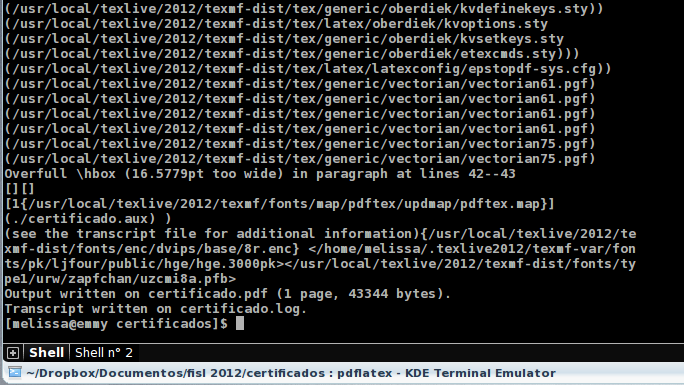
\includegraphics[width=2cm]{imagens/terminal.png}};
         \node<3-> [below of=dummy] (pdf) {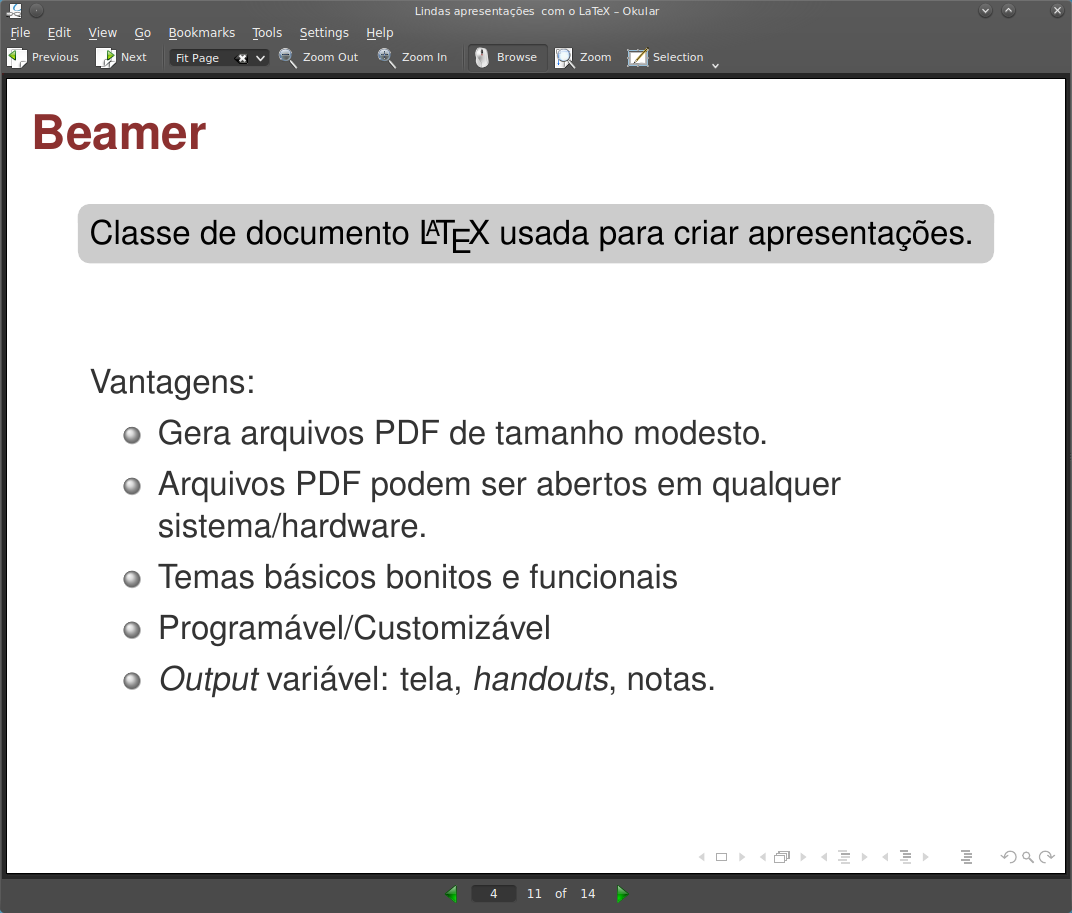
\includegraphics[width=2.5cm]{imagens/output.png}};
         \path<2->[->] (editor.east) edge [bend left] (terminal.north);
         \path<3->[->] (terminal.south) edge [bend left] (pdf.east);
      \end{tikzpicture}
   \end{columns}
\end{frame}

\begin{frame}
   \frametitle{Estrutura básica de um documento}
   \begin{minipage}{0.2\textwidth}
         \begin{tikzpicture}[overlay,scale=0.5]
            % Para ajudar a fazer os gráficos
            %\draw[step=0.5,black,thin,xshift=0.5cm,yshift=0.5cm] (0,-7) grid (4.5,7);
            \draw<3>[very thick, handsomedevil] (4.5,6.5) to (4.15,6.5);
            \draw<3>[very thick, handsomedevil] (4.2,6.5) to (4.2,2.95);
            \draw<3>[very thick, handsomedevil] (4.5,3.0) to (4.2,3.0);
            \node<3>[handsomedevil] at (2,4.9) {Preâmbulo};
            % 
            \draw<6>[very thick, handsomedevil] (4.5,1.8) to (4.15,1.8);
            \draw<6>[very thick, handsomedevil] (4.2,1.8) to (4.2,-0.8);
            \draw<6>[very thick, handsomedevil] (4.5,-0.75) to (4.2,-0.75);
            \node<6>[handsomedevil] at (2,0.5) {Slide título};
         \end{tikzpicture}
      \end{minipage}
      \setbeamercovered{transparent,again covered={\opaqueness<1->{25}}}
      \begin{minipage}{0.75\textwidth}
         \begin{overlayarea}{\textwidth}{0.8\textheight}
            \uncover<1-3,8>{\tt{\kw{documentclass}}\{beamer\}\\}
            \uncover<2-3,8>{\tt{\kw{title}\{Titulo\}\\
                  \kw{author}\{Seu nome\}\\
                  \kw{date}\{Hoje\}}\\}
            \uncover<4->{\tt{\kw{begin}\{document\}}\\}
            \uncover<5->{\tt{\kw{begin}\{frame\}\\
                        \hspace{0.5cm}\kw{titlepage}\\
                        \kw{end}\{frame\}\\}}
            \uncover<7->{\tt{\kw{begin}\{frame\}\\
                        \hspace{0.5cm}\kw{frametitle}\{Titulo do meu slide\}\\
                        \hspace{0.5cm}Texto do meu slide!\\
                        \kw{end}\{frame\}}\\}
            \uncover<4->{\tt{\kw{end}\{document\}}}
         \end{overlayarea}
      \end{minipage}
\end{frame}

\subsection{Ferramentas}

\begin{frame}[fragile]
   \frametitle{Ambientes básicos}
   \begin{columns}
      \column{4cm}
      Texto!
      \begin{block}{Aqui temos um}
         Bloco. \alert{Alerta}
      \end{block}

      \begin{alertblock}{Cuidado!}
         Muito cuidado!
      \end{alertblock}
      \column{6cm}
      \begin{lstlisting}[frame=single,gobble=9]
         Texto!
         \begin{block}{Aqui temos um}
            Bloco. \alert{Alerta}
         \end{block}
         
         \begin{alertblock}{Cuidado!}
            Muito cuidado!
         \end{alertblock}
      \end{lstlisting}
   \end{columns}
\end{frame}

\begin{frame}[fragile]
   \frametitle{Elementos dinâmicos}
   \only<1-5>{\vspace*{3cm}\begin{center}
      \begin{block}{}
         \begin{center}
            \setbeamercovered{transparent}
            \uncover<5->{Podemos} \uncover<2->{definir} \uncover<3->{ambientes} \uncover<4->{dinâmicos} \uncover<5->{!}
         \end{center}
      \end{block}
   \end{center}}
%
   \begin{center}
      \begin{overlayarea}{\textwidth}{\textheight}
         \begin{itemize}
            \setbeamercovered{invisible}
            \item<6-> {\tt{\kw{uncover}<x->\{Texto\}}}
            \item<11-> {\tt{\kw{only}<x->\{Texto\}}} ou {\tt{\kw{invisible}<x->\{Texto\}}}
            \item<16-> {\tt{\kw{alt}<x>\{Texto em x\}\{Texto em outro slide\}}}
            \item<19-> {\tt{\kw{temporal}<x>\{Antes\}\{Em x\}\{Depois\}}}
         \end{itemize}
         \only<6-10>{
         \begin{columns}
            \column{5cm}
            \lstset{frame=single,literate={ê}{{\^e}}1}
            \lstinputlisting{extras/uncover.tex}
            \column{4cm}
            \footnotesize{\noindent%
            \uncover<8->{dois}\\
            \uncover<7->{um}\\
            \uncover<10>{quatro}\\
            \uncover<9->{três}}
         \end{columns}
         \vspace{0.2cm}
         \begin{center}
         \footnotesize{\only<7>{Slide 1}\only<8>{Slide 2}\only<9>{Slide 3}\only<10>{Slide 4}}
         \end{center}
         }
         \only<11-15>{
         \begin{columns}
            \column{5cm}
            \lstset{frame=single,literate={ê}{{\^e}}1}
            \lstinputlisting{extras/only.tex}
            \column{4cm}
            \footnotesize{\noindent%
            \uncover<13>{dois}\\
            \uncover<12-13>{um}\\
            \uncover<15>{quatro}\\
            \uncover<14->{três}}
         \end{columns}
         \vspace{0.2cm}
         \begin{center}
         \footnotesize{\only<12>{Slide 1}\only<13>{Slide 2}\only<14>{Slide 3}\only<15>{Slide 4}}
         \end{center}
         }
         \only<16-18>{
         \begin{columns}
            \column{7cm}
            \lstset{frame=single,literate={ã}{{\~a}}1}
            \lstinputlisting{extras/alt.tex}
            \column{3cm}
            \footnotesize{\alt<17>{\bfseries{Estou no dois!}}{Não estou no dois.}}
         \end{columns}
         \vspace{0.2cm}
         \begin{center}
         \footnotesize{\only<16>{Slide 1}\only<17>{Slide 2}\only<18>{Slide 3}}
         \end{center}
         }
         \only<19-21>{
         \begin{columns}
            \column{6cm}
            \lstset{frame=single}
            \lstinputlisting{extras/temporal.tex}
            \column{3cm}
            \footnotesize{\temporal<20>{Antes do dois...}{\bfseries{Estou no dois!}}{Passei do dois...}}
         \end{columns}
         \vspace{0.2cm}
         \begin{center}
         \footnotesize{\only<19>{Slide 1}\only<20>{Slide 2}\only<21>{Slide 3}}
         \end{center}
         }
      \end{overlayarea}
   \end{center}
\end{frame}

\begin{frame}[fragile]
   \frametitle{Listas}
   \begin{columns}
      \column{5cm}
      \lstset{frame=single,literate={ê}{{\^e}}1}
      \lstinputlisting{extras/listapause.tex}
      \column{5cm}
      \begin{itemize}
         \item Um
         \pause
         \item Dois
         \pause
         \item Três
         \pause
         \item Quatro
      \end{itemize}
   \end{columns}
\end{frame}
\begin{frame}[fragile]
   \frametitle{Listas}
   \begin{columns}
      \column{5cm}
      \lstset{frame=single,literate={ê}{{\^e}}1}
      \lstinputlisting{extras/listasimples.tex}
      \column{5cm}
      \begin{itemize}
         \item<1-> Um
         \item<2-> Dois
         \item<3-> Três
         \item<4-> Quatro
      \end{itemize}
   \end{columns}
   \begin{center}
      \only<1>{Slide 1}\only<2>{Slide 2}\only<3>{Slide 3}\only<4>{Slide 4}
   \end{center}
\end{frame}
\begin{frame}[fragile]
   \frametitle{Listas}
   \begin{center}
      {\tt{\kw{setbeamercovered}\{transparent|invisible\}}}
   \end{center}
   \begin{columns}
      \column{5cm}
      \lstset{frame=single,literate={ê}{{\^e}}1}
      \lstinputlisting{extras/listaincr.tex}
      \column{5cm}
      \setbeamercovered{transparent}
      \begin{itemize}[<+->]
         \item Um
         \item Dois
         \item Três
         \item Quatro
      \end{itemize}
   \end{columns}
   \begin{center}
      \only<1>{Slide 1}\only<2>{Slide 2}\only<3>{Slide 3}\only<4>{Slide 4}
   \end{center}
\end{frame}
\begin{frame}[fragile]
   \frametitle{Listas}
   \begin{columns}
      \column{6cm}
      \lstset{frame=single,literate={ê}{{\^e}}1}
      \lstinputlisting{extras/listahigh.tex}
      \column{4cm}
      \begin{itemize}[<+-|alert@+>]
         \item Um
         \item Dois
         \item Três
         \item Quatro
      \end{itemize}
   \end{columns}
   \begin{center}
      \only<1>{Slide 1}\only<2>{Slide 2}\only<3>{Slide 3}\only<4>{Slide 4}
   \end{center}
\end{frame}

% Novo macro para definir itens coloridos
\def\hilite<#1>
{%
   \temporal<#1>{\color{grrey}}{\color{submerged}}%
   {\color{submerged!25}}
}
\begin{frame}[fragile]
   \frametitle{Listas}
   \begin{columns}
      \column{6cm}
      \lstset{frame=single,literate={ê}{{\^e}}1}
      \lstinputlisting{extras/listatemp.tex}
      \column{4cm}
      \begin{itemize}
         \hilite<1> \item Um
         \hilite<2> \item Dois
         \hilite<3> \item Três
         \hilite<4> \item Quatro
      \end{itemize}
   \end{columns}
   \begin{center}
      \only<1>{Slide 1}\only<2>{Slide 2}\only<3>{Slide 3}\only<4>{Slide 4}
   \end{center}
\end{frame}

\subsection{Imagens}

\begin{frame}
   \frametitle{Figuras}
   \begin{overlayarea}{\textwidth}{\textheight}
      \lstset{frame=single}
      \lstinputlisting{extras/graficos.tex}
      \begin{center}
         \includegraphics<1>[width=1cm]{imagens/tux.png}
         \includegraphics<2>[width=4cm]{imagens/tux.png}
         \includegraphics<3>[width=4cm,angle=90]{imagens/tux.png}
         \includegraphics<4>[width=4cm,%
            trim=10mm 80mm 20mm 5mm,clip]{imagens/tux.png}
      \end{center}
   \end{overlayarea}
\end{frame}

\begin{frame}[fragile]
   \frametitle{Zoom}
   \framezoom<1><2>[border](4.7cm,3cm)(1cm,0.8cm)
   \framezoom<1><3>[border](2.5cm,4cm)(1cm,0.8cm)
   \begin{center}
      
\includegraphics[width=6cm]{imagens/penelope.jpg}
   \end{center}
   \lstset{frame=single}\lstinputlisting{extras/framezoom.tex}
\end{frame}

\begin{frame}
   \frametitle{Colunas}
   \begin{columns}
      \column{0.5\textwidth}
      Para colocar texto e figuras lado a lado, podemos usar o ambiente {\tt{\color{submerged}columns}}.
      \column{0.5\textwidth}
      
\includegraphics[width=4cm]{imagens/barriga.jpg}
   \end{columns}
   \lstset{frame=single}\lstinputlisting{extras/columns.tex}
\end{frame}

\section{Avançado}

\subsection{Temas e cores}

\begin{frame}
   \frametitle{Temas}
   \begin{center}
      {\tt{\kw{usetheme}[option]\{nome\}}}
   \end{center}
   O beamer tem 28 temas pré-definidos em\\
   \begin{center}{\tt{beamertheme<nome>.sty}}\end{center}
\end{frame}

\begin{frame}
   \frametitle{Temas}
   \begin{center}
      {\tt{\kw{usecolortheme}[option]\{nome\}}}\\
   \end{center}
   O beamer tem 17 temas de cores pré-definidos em\\
   \begin{center}{\tt{beamercolortheme<nome>.sty}}\end{center}
\end{frame}

\begin{frame}
   \frametitle{Temas}
   \begin{columns}
      \column{0.5\textwidth}
      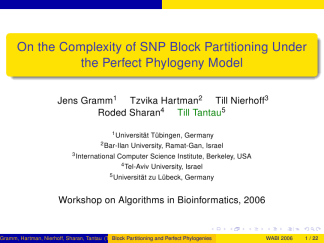
\includegraphics[width=0.45\paperwidth]{imagens/AnnArbor01.png}
      \column{0.5\textwidth}
      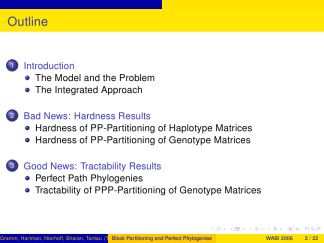
\includegraphics[width=0.45\paperwidth]{imagens/AnnArbor02.png}
   \end{columns}
\end{frame}
\begin{frame}
   \frametitle{Temas}
   \begin{columns}
      \column{0.5\textwidth}
      
\includegraphics[width=0.45\paperwidth]{imagens/Berlin01.png}
      \column{0.5\textwidth}
      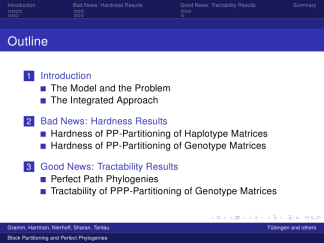
\includegraphics[width=0.45\paperwidth]{imagens/Berlin02.png}
   \end{columns}
\end{frame}
\begin{frame}
   \frametitle{Temas}
   \begin{columns}
      \column{0.5\textwidth}
      
\includegraphics[width=0.45\paperwidth]{imagens/Bergen01.png}
      \column{0.5\textwidth}
      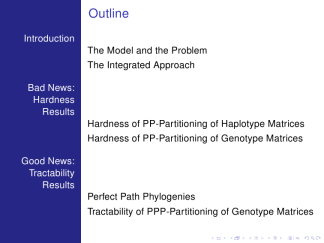
\includegraphics[width=0.45\paperwidth]{imagens/Bergen02.png}
   \end{columns}
\end{frame}
\begin{frame}
   \frametitle{Temas}
   \begin{columns}
      \column{0.5\textwidth}
      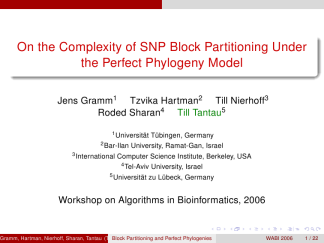
\includegraphics[width=0.45\paperwidth]{imagens/CambridgeUS01.png}
      \column{0.5\textwidth}
      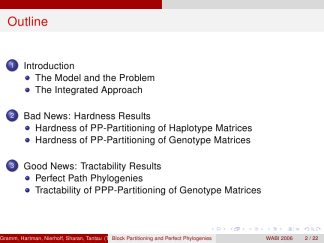
\includegraphics[width=0.45\paperwidth]{imagens/CambridgeUS02.png}
   \end{columns}
\end{frame}
\begin{frame}
   \frametitle{Temas}
   \begin{columns}
      \column{0.5\textwidth}
      
\includegraphics[width=0.45\paperwidth]{imagens/Goettingen01.png}
      \column{0.5\textwidth}
      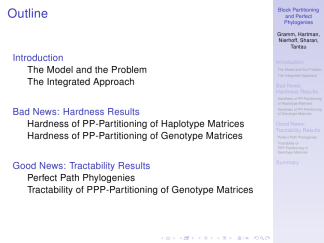
\includegraphics[width=0.45\paperwidth]{imagens/Goettingen02.png}
   \end{columns}
\end{frame}

\begin{frame}
   \frametitle{Customização}
   \lstset{frame=single}
   \lstinputlisting{extras/temas.tex}
\end{frame}

\begin{frame}
   \frametitle{Cores}
   \begin{itemize}
      \item {\tt{\kw{color}\{cor\}}}
      \item {\tt{\kw{usecolortheme}\{tema\}}}
      \item {\tt{\kw{definecolor}\{submerged\}\{rgb\}\{red,green,blue\}}}
      \item {\tt{\kw{setbeamercolor}\{normal text\}\{fg=submerged\}}}
   \end{itemize}
\end{frame}

\subsection{Customização}

{% Background colorido
   \setbeamercolor{normal text}{bg=handsomedevil}
   \setbeamertemplate{footline}{} 
   \setbeamertemplate{headline}{\color{handsomedevil}t}
   \begin{frame}%
      \frametitle{Backgrounds}%
      \vspace{5cm}
      \lstset{frame=single,backgroundcolor=\color{white}}\lstinputlisting{extras/color.tex}%
   \end{frame}
}

{% Background colorido 2
   \setbeamercolor{normal text}{bg=handsomedevil!80!white}
   \setbeamertemplate{footline}{} 
   \setbeamertemplate{headline}{\color{handsomedevil!80!white}t}
   \begin{frame}%
      \frametitle{Backgrounds}%
      \vspace{5cm}
      \lstset{frame=single,backgroundcolor=\color{white}}\lstinputlisting{extras/colorsaturation.tex}%
   \end{frame}
}

{% Background gradiente
   \setbeamertemplate{background canvas}[vertical shading][bottom=handsomedevil,top=white]
   \setbeamertemplate{footline}{}
   \setbeamertemplate{headline}{}
   \begin{frame}%
      \frametitle{Backgrounds}%
      \vspace{5cm}
      \lstset{frame=single,backgroundcolor=\color{white}}\lstinputlisting{extras/colorgradient.tex}%
   \end{frame}
}

\begin{frame}
   \frametitle{Sumário}
   Podemos definir seções e subseções para organizar uma apresentação longa.
   \begin{itemize}
      \item {\tt{\kw{section}\{Seção\}}}
      \item {\tt{\kw{subsection}\{Subseção\}}}
   \end{itemize}      
   \begin{center}
      \lstset{frame=single}\lstinputlisting{extras/toc.tex}
   \end{center}
\end{frame}

\begin{frame}
   \frametitle{Oi eu sou o roteiro!}
   \tableofcontents
   \begin{center}
      {\tt{\kw{tableofcontents}}}
   \end{center}
\end{frame}

\begin{frame}
   \frametitle{Contadores de slides}
   Podemos dizer que estamos no slide 
   \begin{center}
      \insertframenumber\ de \inserttotalframenumber
   \end{center}
   com os comandos
   \begin{center}
      {\tt{\kw{insertframenumber}}} de {\tt{\kw{inserttotalframenumber}}}
   \end{center}
\end{frame}

\subsection{TikZ}

\begin{frame}
   \frametitle{TikZ}
   \begin{center}
      \begin{minipage}{8cm}
         \begin{alertblock}{}
            \begin{center}
               \mbox{}\\"TikZ ist kein Zeichenprogramm" \\("TikZ não é um programa para desenhar")\\\mbox{}
            \end{center}
         \end{alertblock}
      \end{minipage}
   \end{center}
\end{frame}

\begin{frame}
   \frametitle{TikZ}
   \begin{columns}
      \column{0.3\paperwidth}
      {\scriptsize{
            % Definir estilos de bloco
            \tikzstyle{decision} = [diamond, draw, fill=blue!20, text width=4.5em, text centered, node distance=1.6cm, inner sep=0pt]
            \tikzstyle{block} = [rectangle, draw, fill=blue!20, text width=5em, text centered, rounded corners]
            \tikzstyle{line} = [draw, -latex']
            \tikzstyle{cloud} = [draw, ellipse,fill=red!20, node distance=1.6cm]
            \begin{tikzpicture}[node distance = 1cm, auto, scale=0.6]
               % Nós
               \node [block] (init) {inicializar};
               \node [cloud, left of=init] (dados) {dados};
               \node [block, below of=init] (identify) {identificar modelo};
               \node [block, below of=identify] (evaluate) {avaliar modelo};
               \node [block, left of=evaluate, node distance=1.6cm] (update) {atualizar};
               \node [decision, below of=evaluate] (decide) {o modelo é válido?};
               \node [block, below of=decide, node distance=1.6cm] (stop) {pare};
               \node [block, below of=stop] (teste) {sair};
               % Arestas
               \path [line,dashed] (dados) -- (init);
               \path [line] (init) -- (identify);
               \path [line] (identify) -- (evaluate);
               \path [line] (evaluate) -- (decide);
               \path [line] (decide) -| node [near start] {não} (update);
               \path [line] (update) |- (identify);
               \path [line] (decide) -- node {sim}(stop);
               \path [line] (stop) -- (teste);
            \end{tikzpicture}}}
      \column{0.65\paperwidth}
      \lstset{frame=single,literate={á}{{\'a}}1,basicstyle=\tiny\ttfamily\color{grrey},}\lstinputlisting{extras/tikz.tex}
   \end{columns}
\end{frame}

{% Foto no background
   \usebackgroundtemplate{%
      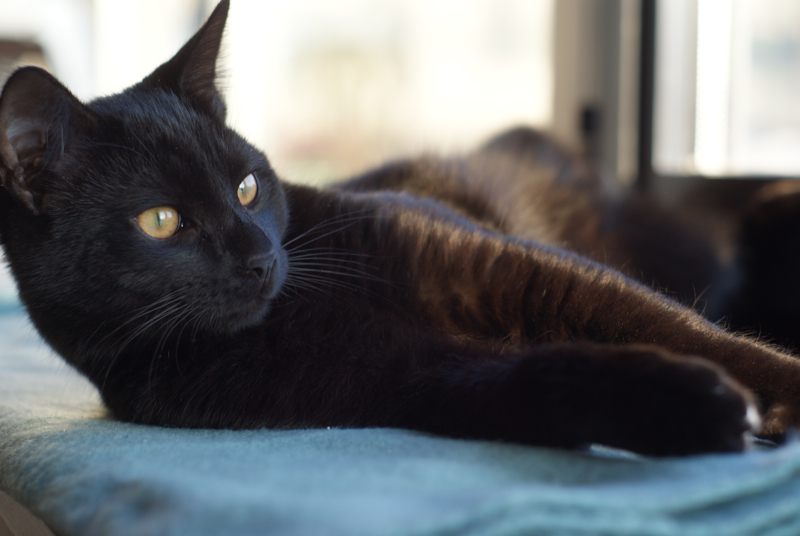
\includegraphics[width=\paperwidth, height=\paperheight]{imagens/linus.jpg}}%
   \begin{frame}%
      \frametitle{Backgrounds}%
      \makebox[\textwidth][c]{
         \begin{tikzpicture}
            \node[fill=white, fill opacity=0.5, text opacity=1] {\lstinputlisting{extras/backtikz.tex}};
         \end{tikzpicture}
      }
   \end{frame}%
}

\begin{frame}[fragile]
   \frametitle{Instalação e mais informações}
   \begin{center}
      \verb+texlive+
   \end{center}
   Mais informações:
   \begin{itemize}
      \item \verb+latex-project.org+
      \item \verb+latexbr.blogspot.com+
      \item \verb+tex.stackexchange.com+
      \item \verb+sourceforge.net/projects/latex-beamer/+
   \end{itemize}

   \begin{center}
      \verb+@melissawm+\\
      \verb+www.mtm.ufsc.br/~melissa+
   \end{center}
\end{frame}

\end{document}